%This section talks about that which is retelling in video games
\section{Retelling games}
% Re-Tellings: The Fourth Layer of Narrative as an Instrument for Critique - Mirjam Palosaari Eladhari
% When the Fourth Layer Meets the Fourth Wall: The Case for Critical Game Retellings - Steven Sych

%This section showcases examples of retelling in video games
\subsection{Examples of TTRPG retellings}
%Adventure Zone (Comic) & Critical Role (Cartoon)

%This section showcases examples 1of AI based retelling/storytelling
\subsection{Artificial Intelligence as a Reteller/storyteller}
%AI Comic factory and The Finals commentator

%In this section we will look at comic studies and use that as a basis for the project
\section{Comic books}
%Understanding Comics (Scott McCloud) and Comics and Sequential Art (Will Eisner)
Making Comic Books is an art form on its own and to understand how to generate a comic book with AI we need to understand how comic books function as an artefact: How they are made; How they are structured; How they are read; And what comic books are. This section will look at comic book studies to create a better understanding of comic book creation.

Comic books are a sequential art form\cite{eisner2008comics}. When you take a comic book panel and look at it outside of the context of other panels it is just an image. But when you place them side by side in a sequential order the pictures become a comic book \ref{fig:SequentialArt}. Looking at the image we can see that an image of a man holding its hat is just a man holding a hat. But when you place two images of a man holding his hat side by side we can see that it creates a motion of tipping his hat. The panels create an effect of change, an effect of time passing. The space between the panels of comic book panels creates a concept of time in stationary images. 

\begin{figure}[!htp]
	\centering
	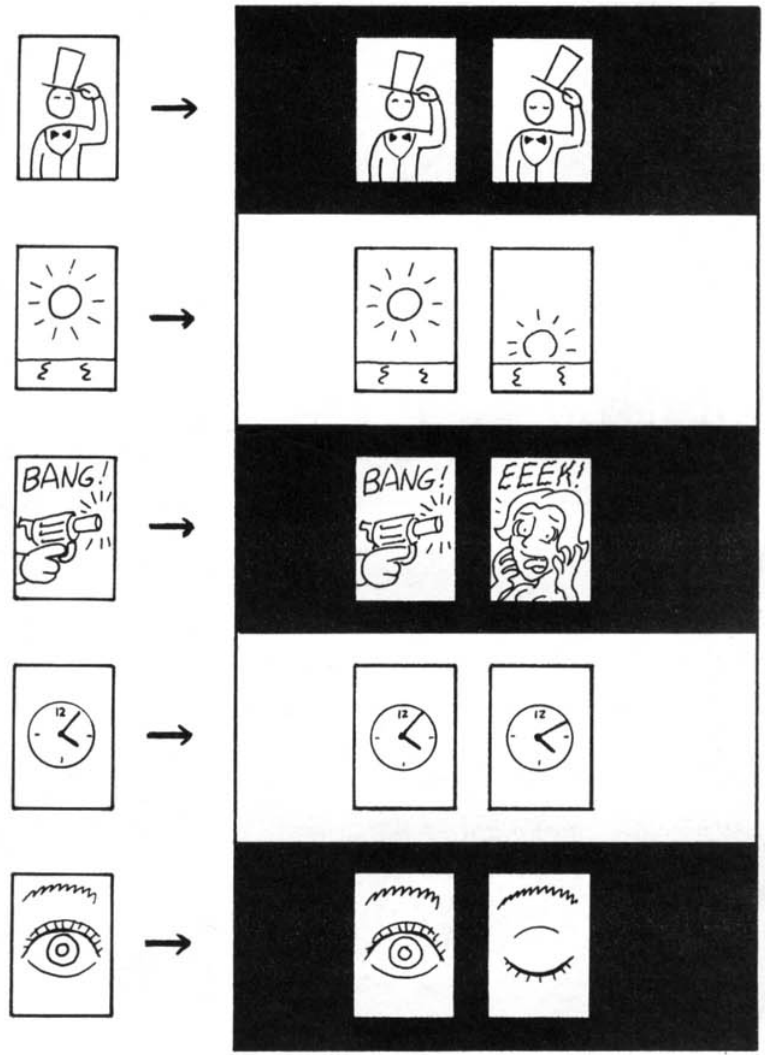
\includegraphics[scale=0.45]{images/SequentalArtUnderstandingComicPage5.png}
	\caption[Sequential Art]{Sequential Art page 5 \cite{mccloud1993understanding}}
	\label{fig:SequentialArt}
\end{figure}

In terms of art style there are many different flavours of comic books. Most people would think of a classic comic book they read as a child. But there are many more. Manga uses grey scale and generally follow a panel structure. American comics mostly are full colour and follow a panel structure. Manhwa/Webcomics are in mostly in full colour but are read from top to bottom by scrolling and are primarily read on the web. And these are just some generic descriptions of comic book art style, there are many unique styles out there like Sin City style (REF) and David Finch's art style (REF). Some comics even break the whole concept of panels and use whole pages as panels. Or place panels in panels. Or have panels that are not rectangular, but crooked, round, bend or anything else (Sandman). And some do not even use panels at all but make use of emptiness or use the same character on a long frame multiple time creating a concept of time as you read left to right. The important take away here is that comic books are not just one style, but many different styles.

Iconography is essential to many comic books to communicate those things that can not be easily spoken or written down. In the world of manga we call this unspoken communication \textit{Manpu} \ref{fig:Iconography}. To quote Matt Alt \textit{ Manpu "speak" what can't be easily spoken (or written) in words} \cite{GigaTown}. "ZZZ" to indicate someone is snoring or sleeping, a circle with starts and birds above a characters head indicate a state of unconsciousness by an impact of sorts, pages being torn of a calendar indicate time passing and one of my favourite making an L with your thumb and index finger and placing it under you chin to indicate deep thought (or the one I do not like where it represent people acting cool). 

\begin{figure}[!htp]
	\centering
	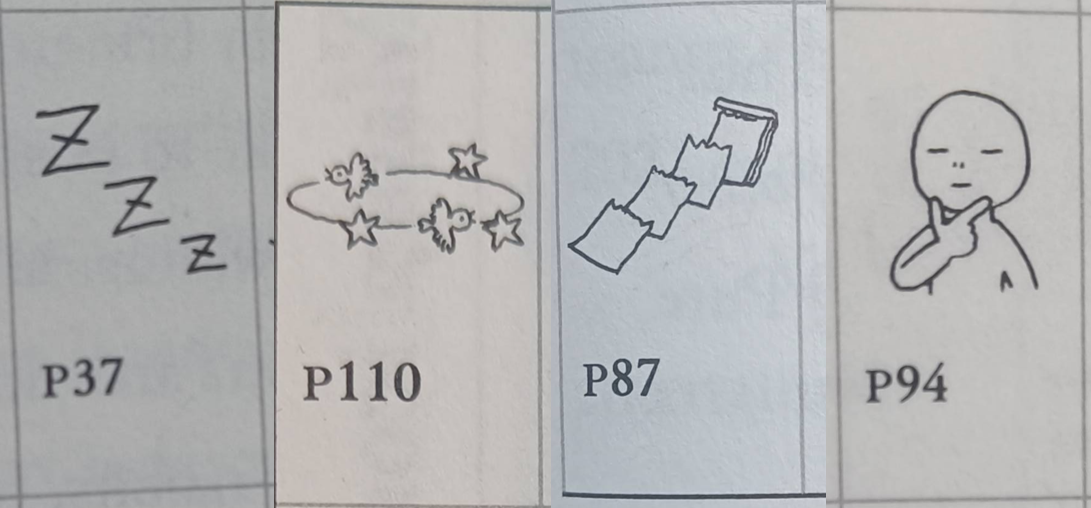
\includegraphics[scale=0.45]{images/IconographyGigaTown.png}
	\caption[Iconography]{Iconography \cite{GigaTown}}
	\label{fig:Iconography}
\end{figure}

Text in comic books are most 


So what did we learn from this? And what can we take with us for the artefact creation?
\begin{enumerate}
    \item Time in comic books. As time passes in between comic book panels we need to make sure that the AI generated comic book has a clear time line. The AI needs to be able to use the time line of the story and how it is told. Connecting panels to each other and create a feeling of time passing.
    \item Different panel styles. As we look at the different styles of panels that comic books use we need to ask ourselves to what extend the panel structure is important in an exploratory retelling artefact of games like the one made for this thesis. The panel structure is primarily an artistic expression of the greater whole of the comic book and the story it tells. The artefact is going to need a structured system to generate panels and it shouldn't have too much freedom to come up with panel structures as this will most likely take away from the retelling of the story of not done very well.
    \item Art start. As 
    \item Text in comic books
    \item Iconography
\end{enumerate}


\subsection{Comic Book take aways}

%In this section we will look at the different AI models and why I chose them
\section{AI models}
There are many different AI models floating around the internet that could be used as part of the artefact that was made for this thesis. To choice which model to use this chapter talks about different models and why they were chosen for this thesis. In the end Mistral has been chosen as the large language model, FLUX.1 has been chosen for the image generation and Whisper has been chosen for the audio transcription model.

The requirements where these models where chosen on were:
\begin{itemize}
	\item Open source
	\item Locally runnable
	\item Good enough performance
	\item Ethical considerations as disclosed in section \ref{AIethics}
\end{itemize}
\subsection{Large Language Models}

Picking a suitable Large Language Model for the project is a quite the impossible task as models keep changing rapidly and new models are released every day. There are many academic papers out there discussing models and their performance, usage and more \cite{2024arXiv240201687A,chang2024survey,hadi2023survey,zhao2023survey}. However all of these are already more than a year old and as models are changing so fast most of those papers are already outdated, however still very useful. As this paper is not an analysis of AI models but a practical thesis I have asked ChatGPT-4-turbo to give me a list of models with their pros and cons and asked it to make me a table for Latex with the information. The prompts that I used: \textit{I would like to have a table with a comparison of the top 10 large language models. Show the pro's and cons of the models. Add if they are open source and locally runnable.} Followed by: \textit{Can you convert that table to Latex code?}. The results can be seen in table \ref{tbl:ModelComparison}, the latex code had to be modified to fit the page.

Even here we can see that the models are out of date. Gemini 1.5 Pro is not the latest model as Gemini 2.5 is already released, and LLaMA 3.1 is not the latest model as LLaMA 4 is already released. However, the table does give a good overview of the models that are available and their pros and cons. Primarily the question if they are open source and can be run locally. I used this method not because I see it as a academic valuable method but because I want to use technology and see how useful it could be for academia. Looking at this small experiment we can see that it could be useful, however the data is very outdated and not very useful. It does point us in the correct direction and gives us a good overview of the models that are available.

\begin{table}[ht!]
\centering
\resizebox{\textwidth}{!}{%
\begin{tabular}{|l|l|p{5cm}|p{5cm}|c|c|}
\hline
\textbf{Model Name} & \textbf{Developer} & \textbf{Pros} & \textbf{Cons} & \textbf{Open Source} & \textbf{Locally Runnable} \\
\hline
GPT-4o & OpenAI & 
Multimodal (text, image, audio); fast and versatile & 
Occasional hallucinations; high compute needed & 
No & No \\
\hline
Claude 3.5 Sonnet & Anthropic & 
Safety-focused; handles long contexts; natural responses & 
Slower; closed API only & 
No & No \\
\hline
Gemini 1.5 Pro & Google DeepMind & 
Strong multimodal support; integrates Google ecosystem & 
Resource-heavy; limited open variants & 
No & No \\
\hline
LLaMA 3.1 & Meta AI & 
Open-source; good at translation and code & 
Requires technical expertise; energy-intensive & 
Yes & Yes \\
\hline
Mistral Large 2 & Mistral AI & 
Strong reasoning and code generation; long contexts & 
Commercial license; proprietary & 
No & Limited (license) \\
\hline
DeepSeek-R1 & DeepSeek & 
Multilingual support; efficient & 
Limited adoption; less documented & 
No & No \\
\hline
Mixtral & Mistral AI & 
Efficient Mixture of Experts; open-source & 
Shorter context; niche usage & 
Yes & Yes \\
\hline
Grok 3 & xAI & 
Good social media integration; open-source focus & 
Requires subscription; limited distribution & 
Yes & Possibly (limited) \\
\hline
Command R+ & Cohere & 
Up-to-date info retrieval; good conversational skills & 
Limited multimodal support & 
No & No \\
\hline
Phi-2 & Microsoft & 
Open-source; efficient size/performance & 
Limited multimodal support; some bias concerns & 
Yes & Yes \\
\hline
\end{tabular}
}
\captionof{table}{Comparison table of 10 LLM's by ChatGPT-4-turbo}\label{tbl:ModelComparison}
\end{table}\noindent

Looking at the options provided we can quickly cut out most of the models as they are not open source and there is no possibility of running them locally. The models that are left are LLaMA, Mixtral and Phi. Out of these 3 models the choice is easy as Mixtral is the only options. Even do the other two models are open source, they are still owned by large American corporations (Microsoft and Meta) which are from personal point of view out of the question to use (More on this in \ref{AIethics}). Mistral is an privately owned and French company.

\subsection{Image generation models} 

\cite{bie2024renaissance}

%Talk about Stable Diffusion, Llama 3.1-8B and Whisper and why I chose them. Also talk about other models and why I did not choose them.

%In this section I will talk about the ethical consideration around AI usage.
\section{AI ethics} \label{AIethics}
Hello
%The Ethics of AI in games. – Melhart et al.
% Building ethics into artificial intelligence. – Yu et al.
% Deep Learning for Coders with Fastai and Pytorch: AI Applications Without a PhD – Jeremy Howard & Sylvain Gugger
% The ethics of Artificial Intelligence – Nick Bostrom & Eliezer Yudkowsky
% Think about stepping on the toes of artists and writers.

\section{The art of AI prompting}
Writing AI prompts is not something you can properly do without thinking about it. Writing proper prompts is a lot like writing code where you need to iterate over the instructions you give the computer to do what you want it to do. It is also know as prompt engineering. There are a lot of nuances to writing prompts and hidden tricks and commands to instruct an AI to get an AI to do exactly what you want it to do. This section discusses the basics of AI prompting and how they have been used in the artefact.

\cite{dang2022prompt}
%https://scholar.google.com/scholar?hl=nl&as_sdt=0%2C5&q=How+to+prompt+ai&btnG=